\documentclass{article}
\usepackage{graphicx} % Required for inserting images
\usepackage{amsmath, bm, mathtools, amsfonts, amssymb}
\usepackage{xcolor}
\usepackage{adjustbox} 
\usepackage{hhline}
\usepackage{caption}
\captionsetup[table]{position=bottom} 
\usepackage{array, makecell}
\newcommand*{\vertbar}{\rule[-1ex]{0.5pt}{2.5ex}}
\newcommand*{\horzbar}{\rule[.5ex]{2.5ex}{0.5pt}}
\newcommand{\diff}{\mathop{}\!\mathrm{d}}

\usepackage{tikz}
\usetikzlibrary{decorations.pathreplacing,calligraphy}
\usetikzlibrary{positioning}
\usetikzlibrary{positioning,shapes.symbols,fit}
\tikzset{
	roundnode2/.style={circle, draw=green!50!blue, very thick, minimum size=9mm}
}
%\usetikzlibrary{shapes, arrows, calc, arrows.meta, fit, positioning}
%\usetikzlibrary{arrows.meta}
\tikzset{
	roundnode/.style={circle, draw=green!50!blue, fill=green!60!blue, very thick, minimum size=7mm},
	rectnode/.style={rectangle, draw=green!50!blue, very thick, minimum size=8.5mm},
	mydotted/.style = {dash pattern=on 6.1pt off 7pt}
}


%\usepackage[backend=bibtex,style=numeric,natbib=true,maxbibnames=5,giveninits=true]{biblatex}
\usepackage[backend=bibtex,style=numeric,natbib=true,maxbibnames=5,giveninits=true]{biblatex}
\newcommand*{\bibtitle}{References}
\DeclareNameAlias{default}{last-first}
\addbibresource{bib.bib}

\title{Tensor-Train Paper}
\author{Lennart}
\date{November 2025}

\begin{document}

\maketitle

\section{Introduction}
\begin{itemize}
	\item Hierarchical Bayesian modelling including Pressure and Temperature
    \item Forward model ozone limb-sounding as linear inverse problem
    \item Marginal and full conditional posterior explicitly formulated
    \item samples from full conditional posterior via IRT
    \item sample-based affine map
    \item same procedure again
    \item full posterior mean and sample-based variance do not capture second ozone peak
    \item Pressure and Ozone highly correlated
    \item All programming and analysis in this thesis are done in Python, and the reported computation times are taken on a MacBook Pro from 2019 with a 2.4 GHz quad-core Intel i5 processor.
\end{itemize}
\section{Linear inverse Problem --  Hierarchical Bayesian Modelling}
\label{sec:BayesIntro}
First the concept of hierarchical Bayesian modelling is introduced.
Assume we observe some data
\begin{align}
	\bm{y} = \bm{A} \bm{x} + \bm{\eta},
	\label{eq:NonLinDat}
\end{align}
based on a linear forward model $\bm{A}$ an unknown parameter vector $\bm{x}$ and some additive random noise $\bm{\eta}$.
Naturally, due to the noise, the observation process in Eq. \ref{eq:NonLinDat} is a random process.
Hence, in Bayesian modelling, the aim is to determine a probability distribution over the parameter $\bm{x}$ given some data $\bm{y}$.
Further, a hierarchical Bayesian model incorporates (auxiliary) hyper-parameters $\bm{\theta}$.
Within a Bayesian approach all unknown hyper-parameters and parameters are treated as random variables \cite[Chapter 3]{kaipio2005statinv}.

According to Bayes' theorem, the joint posterior distribution over the parameters $\bm{x}$ and the hyper-parameter $\bm{\theta}$ is given as
\begin{align}
	\pi(\bm{x},\bm{\theta}|\bm{y}) = \frac{ \pi(\bm{y} | \bm{x}, \bm{\theta} ) \pi(\bm{x}, \bm{\theta})}{\pi(\bm{y})} \propto \pi(\bm{y} | \bm{x}, \bm{\theta} ) \pi(\bm{x}, \bm{\theta}) \, ,
\end{align}
with finite and non-zero $\pi(\bm{y})$.
The likelihood function $\pi(\bm{y}|\bm{x},\bm{\theta})$ is defined by the nature of the noise and the noise-free data $\bm{A}\bm{x}$, which we read as the distribution over $\bm{y}$ conditioned on $\bm{x}$ and $\bm{\theta}$.
Here $\bm{\theta}$ describe multiple hyper-parameters, e.g.~the noise precision so that $\bm{\eta} \sim \pi_{\bm{\eta}}(\cdot|\bm{\theta})$, where $\sim$ reads as ``is distributed as''.
Further, $\bm{\theta}$ may account for some physical properties of $\bm{x}$ such as the smoothness (see Sec.~\ref{sec:BayModel}).
Because all unknown parameter are treated as random variables the joint prior distribution is introduced as $\pi(\bm{x}, \bm{\theta}) = \pi(\bm{x}|\bm{\theta}) \pi(\bm{\theta})$ with the parameter prior distribution $\pi(\bm{x}|\bm{\theta})$ and the hyper-prior distribution $\pi(\bm{\theta})$.
Choosing these prior distributions is ultimately a modeller's choice and is crucial, as those shall be as uninformative as possible for regions in hyper-parameter and parameter space where the data is informative.
If the data is uninformative, the prior distributions can be informative and may represent a rather restrictive range of (physically) feasible hyper-parameters and parameters.

We can write the hierarchical model as:
\begin{subequations}
	\begin{align}
		\bm{y} |  \bm{x},\bm{\theta}  &\sim \pi(\bm{y} | \bm{x}, \bm{\theta} ) \\
		\bm{x}| \bm{\theta}   &\sim \pi(\bm{x}|\bm{\theta})   \\
		\bm{\theta}   &\sim \pi(\bm{\theta} ) \, .
	\end{align} 
\end{subequations}
Usually, the objective is to calculate the expectation of a function $h(\bm{x})$, which is defined as
\begin{align}
	\text{E}_{\bm{x},\bm{\theta}|\bm{y}} [h(\bm{x})] =  \int \int   h(\bm{x}) \,  \pi(\bm{x}, \bm{\theta} | \bm{y} ) \, \diff \bm{x}  \, \diff \bm{\theta}  \label{eq:expPos} \, .
\end{align}
\subsection{Marginal and then Conditional Method}
\label{subsec:TheoMTC}
Characterising the posterior distribution or quickly generating a representative sample set from the posterior distribution often presents a significant challenge. 
This is mainly due to the strong correlations that usually exist between the parameters $\bm{x}$ and hyper-parameters $\bm{\theta}$, as discussed by Rue and Held in~\cite{rue2005gaussian}.

Depending on the problem and the available model it is beneficial to factorise the joint posterior distribution
\begin{align}
	\pi(\bm{x}, \bm{\theta} |  \bm{y}) = \pi(\bm{x} |  \bm{\theta}, \bm{y}) \, \pi(\bm{\theta} |   \bm{y}) \label{eq:MTC}
\end{align}
into the full conditional posterior $\pi(\bm{x} |  \bm{\theta}, \bm{y})$ over the latent field $\bm{x}$ and the marginal posterior $ \pi(\bm{\theta} |   \bm{y})$ over hyper-parameter $\bm{\theta}$.
This approach, known as the marginal and then conditional (MTC) method~\cite{fox2016fast}, is particularly advantageous when $\bm{x}\in \mathbb{R}^n$ is high-dimensional, while $\bm{\theta}$ is low-dimensional and the evaluation of the marginal posterior
\begin{align}
	\pi(\bm{\theta} |   \bm{y}) =  \frac{ \pi(   \bm{y} | \bm{x},\bm{\theta})  \pi( \bm{x} | \bm{\theta} )  \pi(\bm{\theta}) }{ \pi(\bm{x} | \bm{\theta} ,   \bm{y})   \pi( \bm{y})} \propto \frac{ \pi(   \bm{y} | \bm{x},\bm{\theta})  \pi( \bm{x} | \bm{\theta} )  \pi(\bm{\theta}) }{ \pi(\bm{x} | \bm{\theta} ,   \bm{y}) } \label{eq:margGen}\, 
\end{align}
as in~\cite[Lemma 2]{fox2016fast} is relatively cheap.

Applying the law of total expectation~\cite{champ2022generalizedlawtotalcovariance}, Eq.~\eqref{eq:expPos} becomes
\begin{align}
	\mathbb{E}_{\bm{x} ,\bm{\theta}  |\bm{y}} [h(\bm{x})] &= \int \int   h(\bm{x}) \pi(\bm{x} |  \bm{\theta}, \bm{y}) \, \diff \bm{x} \,  \pi(\bm{\theta} |   \bm{y}) \, \diff \bm{\theta} \\
	&= \int \mathbb{E}_{\bm{x} |  \bm{\theta}, \bm{y}} \left[ h(\bm{x}) \right] \, \pi(\bm{\theta} |  \bm{y}) \, \diff \bm{\theta}\label{eq:2fullCond} \\
		&= \mathbb{E}_{\bm{\theta} |  \bm{y}} \left[ \mathbb{E}_{\bm{x} |  \bm{\theta}, \bm{y}} [h(\bm{x})] \right] \, .
	\label{eq:fullCond}
\end{align}
In the case of a linear-Gaussian hierarchical Bayesian model, both the marginal distribution $\pi (\bm{\theta}| \bm{y})$ 
and the inner expectation $\mathbb{E}_{\bm{x} |  \bm{\theta}, \bm{y}} \left[ h(\bm{x}) \right]$ are well defined (see Sec.~\ref{sec:BayModel}).
If the integral in Eq.~\ref{eq:2fullCond} is expensive to calculate  sample-based methods may be used to calculate the expectations in 
Eq.~\eqref{eq:2fullCond}.
To produce a samples $\{ (\bm{x}, \bm{\theta})^{(1)}, \dots, (\bm{x}, \bm{\theta})^{(k)}, \dots, (\bm{x}, \bm{\theta})^{(N)} \} \sim \pi(\bm{x}, \bm{\theta} |  \bm{y}) $ one needs an independent an sample from $\bm{\theta}^{(k)} \sim \pi(\bm{\theta} |  \bm{y})$ first and then draw a sample from the full conditional posterior $\bm{x}^{(k)} \sim \pi(\bm{x} | \bm{\theta}^{(k)}  , \bm{y})$.
\clearpage

\section{The Forward Model}
\label{ch:formodel}
Here we present the forward model to which we apply the methodology.
The forward model describes a Limb-sounder measuring thermal radiation of ozone to determine the atmospheric ozone concentration.
We follow the MIPAS handbook~\cite{mipas2000handbook} and simulate data according to an idealised cloud-free atmosphere in local thermodynamic equilibrium, assuming a measurement instrument with infinite spectral resolution and no pointing errors.
This is a simplified forward model.
No other instrument-specific details such as sensor area or antenna response are included because they are not available to us. 

\begin{figure}[ht!]
	\centering
	\input{LIMB.pdf_tex}
	\caption[Schematic of measurement and analysis geometry.]{Schematic of measurement and analysis geometry, not to scale.
		The stationary satellite, at a constant height $h_\text{sat}$ above Earth, takes $m$ measurements along its line-of-sight defined by the line $\Gamma_j$.
		Each measurement has a pointing angle $\phi_j$ and a tangent height $h_{\ell_j}$, $j=1,2,\dots,m$ defined as the closest distance of $\Gamma_j$ to the Earth's surface.
		Between $h_{L,0} \approx 7$km and $h_{L,n} \approx 83$km, the atmosphere is discretised into $n$ layers as illustrated by the solid green lines.}
	\label{fig:LIMB}
\end{figure}
As displayed in Fig.~\ref{fig:LIMB}, a satellite at a constant height $h_{\text{sat}}$ is pointing through the atmosphere (limb-sounding) to measure thermal radiation of ozone.
For each measurement $j=1,2,\ldots,m$, the tangent height $h_{\ell_j}$ and the corresponding line-of-sight $\Gamma_j$ are defined.
Additionally, we introduce the pointing angle $0 \leq \phi_j < \phi_{\text{max}}$, so that if $\phi = 0 \text{arc sec}$ the satellite points at $h_{L,0}$ and for a pointing angle $\phi_{\text{max}}$ at $h_{L,n}$.
Further, the atmosphere is discretised into $n$ layers defined by height values $h_{L,i-1} < h_{L,i}$ with respect to the surface of the Earth, for $i = 1, \dots, n$.
More specifically, the $i$-th layer is defined by two spheres around the centre of the Earth with radii $ r_0 + h_{L,i-1} $ and $r_0 + h_{L,i}$, where $r_0$ is the Earth's radius.
Within a layer the signal is constant, whereas above $h_{L, n}$ and below $h_{L,0} $ no signal can be obtained.


\subsection{Radiative Transfer Equation}
\label{sec:RTE}
One noise-free measurement of thermal radiation emitted by gas molecules within the atmosphere is described by the radiative transfer equation (RTE)~\cite{mipas2000handbook}
\begin{align}
	\label{eq:RTE} 
	  \int_{\Gamma_j}  B(\nu,T) k(\nu, T)   \frac{p(r)}{k_{\text{B}} T(r)}  x(r)  \tau(r) \text{d}r \,  \\
\text{with } \,	\tau(r) = \exp{ \Bigl\{ - \int^{r}_{r_\text{obs}}  k(\nu, T)   \frac{p(r^{\prime})}{k_B T(r^{\prime})}  x(r^{\prime}) \text{d}r^{\prime} \Bigr\} } \, \label{eq:absRTE} .
\end{align}
This is a path integral along the satellite's straight line of sight $\Gamma_j$ with the ozone volume mixing ratio (VMR) $x(r)$ at distance $r$ from the satellite, at the wave number $\nu$.
Within the atmosphere, the number density $p(r) / (k_{\text{B}} T(r))$ of molecules is dependent on the pressure $p(r)$, the temperature $T(r)$, and the Boltzmann constant $k_{\text{B}}$.
The factor $\tau(r)\leq 1$ accounts for re-absorption of the radiation along the line-of-sight, which makes the RTE non-linear.
The absorption constant is given as
\begin{align}
	k(\nu, T) = L(\nu, T_{\text{ref}}) \frac{Q(T_{\text{ref}})}{Q(T)} \frac{ \exp{\{ - c_2 E^{\prime \prime} / T\}} }{\exp{\{ - c_2 E^{\prime \prime} / T_{\text{ref}} \}}} \frac{ 1- \exp{\{ - c_2 \nu  / T \}} }{1 - \exp{\{ - c_2 \nu / T_{\text{ref}} \}}}
\end{align}
with Planck's constant $h$ and speed of light $c$.
The line intensity $L(\nu, T_{\text{ref}})$ at reference temperature $T_{\text{ref}} =296K $, the lower-state energy $ E^{\prime \prime} $ in $\text{cm}^{-1}$ of the targeted transition and the second radiation constant $c_2\coloneqq hc/k_{\text{B}} \approx 1.44\text{cmK}$ are provided by the HITRAN database~\cite{gordon2022hitran2020}.
The total internal partition function is given as
\begin{align}
	Q(T )= g^{ \prime} \exp{\{ - \frac{ c_2 E^{ \prime} }{T}\}} + g^{\prime \prime} \exp{\{ - \frac{ c_2 E^{\prime \prime} }{T}\}} \, ,
\end{align}
with the statistical weight $ g^{\prime \prime}$ for the lower and $ g^{ \prime}$ for the upper energy state (also called the degeneracy factors) accounting for the molecule's non-rotational and rotational energy states (see also~\cite{vsimevckova2006einstein}), and the upper state energy $E^{ \prime} = E^{ \prime\prime} + \nu$.
Under the assumption of local thermodynamic equilibrium (LTE), the black body radiation acts as a source function
\begin{align}
	B(\nu,T)   = \frac{2 h c^2 \nu^3}{\exp{\{\frac{c_2\nu}{ T}\}}-1}\, .
\end{align}
For fundamentals on the RTE, we recommend~\cite[Chapter 1]{rybicki2000rte}, and for a more comprehensive model, we refer to \cite{read2006forwardModel}.

When simulating data, we assume an idealised limb-sounder.
Since the measurement device has a negligible frequency window, the line broadening around $\nu$ for the calculations of $L(\nu, T_{\text{ref}})$ is neglected.
Normally, this is modelled as the convolution of the normalised Lorentz profile (collisional/pressure broadening) and the normalised Doppler profile (thermal broadening)~\cite{mipas2000handbook}.
Additionally, we target one specific molecule and calculate $k(\nu, T)$ accordingly.
Usually, this would involve a summation over the individual absorption constants for multiple radiating molecules weighted by their respective VMR~\cite{mipas2000handbook}.


\subsection{Simulated Data and Ground Truth}
\label{sec:SimDat}
As the ground truth for our methodology, we consider an ozone profile at distinct pressure values generated from some data~\cite{MLSdata} of the MLS on the Aura satellite within the Antarctic region.
This ozone profile has a peak in the middle atmosphere and a second peak at higher altitudes, see Fig.~\ref{fig:OzonSampl}, which seems to be a typical nighttime profile~\cite{Lee2020NightOzone}.
For more information on the processes within the atmosphere for ozone, we refer to~\cite{Lee2020NightOzone}.

We can relate the height $h$ and the pressure values $p$ via the hydrostatic equilibrium equation
\begin{align}
	\text{d}(\log p) = \frac{\text{d}p}{p} = \frac{- g M}{R^* T} \text{d} h \, .\label{eq:hydr}
\end{align}
Here the acceleration due to gravity is $g$, the universal gas constant is $R^* = 8.31432 \times 10^{-3} \text{Nm} / \text{kmol} / \text{K}$ and the mean molecular weight of the air is $M = 28.97 \text{kg/kmol}$, as in~\cite{atmosphere1976us}.
To enable efficient calculation of the RTE we discretise the atmosphere as in Fig.~\ref{fig:LIMB}.
Then the ozone VMR $\bm{x} =\{x_1,x_2,\ldots,x_n\} \in \mathbb{R}^{n}$, pressure $\bm{p} =\{p_1,p_2,\ldots,p_n\} \in \mathbb{R}^{n}$ and temperature $\bm{T} =\{T_1,T_2,\ldots,T_n\} \in \mathbb{R}^{n}$, as well as all other height dependent parameters, are discretised profiles with constant values between the heights $h_{L,i-1} \leq h < h_{L,i}$, for each layer $i = 1,\dots, n$.
The hydrostatic equilibrium equation for the discretised atmosphere is
\begin{align}
	h_{L,i} =  h_{L,i-1} - \frac{\Delta p R^* T_{i-1}  }{p_{i-1}  g_{i-1} M} \, 
\end{align}
with $\Delta p = p_{i} - p_{i-1}$ and $T_{i-1} = T(h_{i-1})$ as in Eq.~\ref{eq:tempFunc} (see also~\cite{Carlotti99,Ridolfi00}), for $i = 1,\dots, n$.
At sea level $h = 0$km the mean pressure is $p_0 = 1013.25$hPa and the mean temperature is $T_0 = 288.15$K~\cite{atmosphere1976us}.
The acceleration due to gravity is
\begin{align}
	g_i = g_0 \Bigg( \frac{r_0}{r_0 + h_{L,i}} \Bigg) \, ,
\end{align}
where the polar radius of the Earth is $r_0 \approx 6356 \, \text{km}$, the gravitation at sea level is $g_0 \approx 9.81 \text{m}/\text{s}^2$.
For a ground truth temperature profile we follow~\cite{atmosphere1976us} and form the temperature function
\begin{equation}
	\label{eq:tempFunc}
	T(h) = \adjustbox{max width=0.825\textwidth}{$\begin{dcases*}
			T_0 &, \text{$h  = 0$}\\
			T_0 + a_0 h   &, \text{$0 \leq h < h_{T,1}$}\\
			T_0 + a_0 h_{T,1} &, \text{$h_{T,1} \leq  h < h_{T,2}$}\\
			T_0 + a_0 h_{T,1} + a_1 (h_{T,2}   - h_{T,1})  + a_2 (h   - h_{T,2})  &, \text{$h_{T,2} \leq h < h_{T,3}$}\\
			T_0 + a_0 h_{T,1} + a_1 (h_{T,2}   - h_{T,1})   & \\
			\hphantom{{} T_0 } + a_2 (h_{T,3}   - h_{T,2}) + a_3 (h   - h_{T,3}) &, \text{$h_{T,3} \leq h < h_{T,4}$}\\
			T_0 + a_0 h_{T,1} + a_1 (h_{T,2}   - h_{T,1})  & \\
			\hphantom{{} T_0 }+ a_2 (h_{T,3}   - h_{T,2})  + a_3 (h_{T,4}   - h_{T,3}) + a_4 (h   - h_{T,4}) &, \text{$h_{T,4} \leq h < h_{T,5}$}\\
			T_0 + a_0 h_{T,1} + a_1 (h_{T,2}   - h_{T,1})   & \\
			\hphantom{{} T_0 } + a_2 (h_{T,3}   - h_{T,2}) + a_3 (h_{T,4}   - h_{T,3}) + a_4 (h_{T,5}   - h_{T,4})& \\
			\hphantom{{} T_0 }  + a_5 (h   - h_{T,5}) &, \text{$h_{T,5} \leq h < h_{T,6}$}\\
			T_0 + a_0 h_{T,1} + a_1 (h_{T,2}   - h_{T,1})    &\\
			\hphantom{{} T_0}  + a_2 (h_{T,3}   - h_{T,2}) + a_3 (h_{T,4}   - h_{T,3}) + a_4 (h_{T,5}   - h_{T,4}) &\\ 
			\hphantom{{} T_0} + a_5 (h_{T,6}   - h_{T,5}) + a_6 (h   - h_{T,6})   &, \text{$h_{T,6} \leq h \lesssim  86$}
		\end{dcases*}$}\\
\end{equation}
with gradient and height values in Tab.~\ref{tab:tempGrad} provided by~\cite{atmosphere1976us}.
This function describes the mean temperature in the atmosphere with various height-depending gradients according to the different atmospheric layers.
This holds up to a geometric height of $86$km, where we ignore a $0.04\%$ non-linear change in $M$ from $80$km to $86$km.
\begin{table}
	\centering
	\begin{tabular}{ |c||c|c|  }
		\hline
		subscript $i$ & geometric height $h_{T,i}$ in km&gradient $a_i$\\
		\hhline{|=||=|=|}
		0& 0 & -6.5\\
		1& 11 & 0\\
		2& 20.1& 1\\
		3& 32.2& 2.8\\
		4& 47.4& 0\\
		5& 51.4& -2.8\\
		6& 71.8& -2\\
		\hline
	\end{tabular}
	\caption[Height depending temperature gradients]{Definition of height depending temperature gradients.}
	\label{tab:tempGrad}
\end{table}

We target ozone at a frequency of $235.71$GHz, which lies within the region where the MLS observes ozone~\cite{livesey2008ozonecarbonmono, waters2006earth}.
The corresponding wave number is $\nu = 7.86\text{cm}^{-1}$.
The absorption constant $k(\nu,T)$ is calculated as in Eq.~\ref{eq:absRTE}, following the high-resolution transmission (HITRAN) database~\cite{gordon2022hitran2020}.
The HITRAN database provides the line intensity $L(\nu,T_{\text{ref}})$ for the isotopologue $\prescript{16}{}{\text{O}}_3$ with the AFGL Code 666.

To compute a data vector, we define an atmosphere between $h_{L,0} = 6.9$km and $h_{L,n} = 83.3$km with $n = 45$ equidistant layers and a satellite fixed at a height of $h_{\text{sat}} = 500$km (see Fig.~\ref{fig:LIMB}).
We measure $m=30$ times between heights of $\approx 7$km and $\approx 68$km with pointing accuracy $175  \text{arc sec}$ and equidistant spaced pointing angles
\begin{align*} 
		\phi_j  =  (j-1) 175 \text{arc sec} ,  \qquad  \text{for } j = 1, \dots, 30\, .
\end{align*}
Above $\approx 68$km the data is noise dominated (see Fig.~\ref{fig:Data}), hence no measurement are taken in larger altitudes.
Each pointing angle $\phi_j$ defines a path $\Gamma_j$ (see Fig.~\ref{fig:LIMB}).
The corresponding path integrals in Eq.~\ref{eq:RTE} and Eq.~\ref{eq:absRTE} are evaluated using the trapezoidal rule and define the non-linear forward model $\bm{A}(\bm{x},  \bm{p},\bm{T})   \in \mathbb{R}^{m}$ for the set of $m$ noise-free measurements.
Here, each entry $A_{j}$ of $\bm{A}(\bm{x},\bm{p},\bm{T})\in \mathbb{R}^{m}$ includes multiple evaluations of the integral in Eq.~\ref{eq:absRTE} to calculate the absorption $\tau(r)$.
For brevity we denote the non-linear forward model as $\bm{A}(\bm{x}) \coloneqq \bm{A}(\bm{x},  \bm{p},\bm{T})$.
The simulated data vector
\begin{align}
	\bm{y} = \bm{A}(\bm{x}) + \bm{\eta}\, 
\end{align}
includes an additive identically-distributed Gaussian noise vector $\bm{\eta} \sim \mathcal{N}(0,\gamma^{-1} \bm{I})$.
The noise precision is chosen so that the signal-to-noise ratio (SNR) is approximately $150$.
The SNR is defined as
\begin{align}
	\text{SNR} \coloneqq \frac{\max(y)}{\text{STD noise}} = \frac{\text{peak signal}}{\text{RMS noise}} \label{eq:SNR} \, ,
\end{align}
where STD noise is the standard deviation of the noise.
An SNR of 150 is similar to~\cite{Froidevaux2008snrozone}, where a signal with a maximal spectral intensity of around $100\text{K}$ and a noise range of $0.4$ to $1.6\text{K}$ is reported.

By neglecting the absorption (e.g., set $\tau = 1$ in Eq.~\eqref{eq:absRTE}) the RTE is linearised.
This denotes the linear forward model matrix $\bm{A}_L\in \mathbb{R}^{m\times n}$.
The integral in Eq.~\eqref{eq:RTE} is evaluated using the trapezoidal rule and enables matrix-vector multiplication $\bm{A}_L \bm{x}$ to compute noise-free linear data.
Since neglecting the absorption changes the measurements only slightly (about $1\%$, see Sec.~\ref{sec:affine}), we classify the inverse problem as a weakly non-linear inverse problem.
Note that the methods used here will work with different SNRs or other frequencies.

\clearpage
\section{Hierarchical Bayesian Model}
\label{sec:BayModel}
Here a hierarchical Bayesian model is developed where the forward model is described by either $\bm{A}_L$ the linearised RTE  (see Eq.~\ref{eq:RTE}) or by the approximation $\bm{M} \bm{A}_L$ to the non-linear RTE, where $\bm{M}$ is an affine map.
Parameters and hyper-parameter are classified and a choice of prior distributions is established.
A directed acyclic graph (DAG) is used to visualise conditional dependencies between hyper-parameters and the parameter (see Fig.~\ref{fig:DAGO3}), as well as how distributions progress through to an observation (square box). 
We plot statistical dependencies as solid arrows and deterministic dependencies as dotted arrows.
Then, applying the MTC scheme, we explicitly formulate the respective posterior distributions.

\subsection{Prior Modelling}
\label{subsec:PriorFull}
First we describe the ozone parameter trough normally distributed prior $\bm{x}| \delta \sim \mathcal{N}(0, \bm{Q}^{-1}) $ with zero mean and no other restrictions, it is clear that our model does not take into account that ozone values cannot be negative.
The precision matrix of that prior distribution is
\begin{align}
	\bm{Q} = \delta \bm{L} =
	\delta
	\begin{bmatrix}
		2 & -1 & & &  \\
		-1 & 2 & -1 & &   \\
		& \ddots & \ddots & \ddots &\\ 
		& & -1 & 2 & -1  \\
		& & & -1 & 2 
	\end{bmatrix} 
	\label{eq:GLapl} 
\end{align}
which is a discrete approximation to the second derivative operator with Dirichlet boundary condition and defines a 1-dimensional Graph Laplacian as in~\cite{wang2015graphs, fox2016fast}, accounting for smoothness in the ozone profile.
We reduce the dimension of $\bm{x}$ from $45$ to $n = 34$ by discarding every second ozone VMR over a height of $\approx47$km.
Doing that, while not changing $\bm{L}$ effectively induces a larger correlation between points at higher altitude.


\begin{figure}[ht!]
	\centering
	\input{TrueTemp.pdf_tex}
	%\includegraphics{PriorTempPostMeanSigm.png}
	\caption[Prior Samples of $\bm{T}$ according to the respective hyper-prior distribution.]{Prior samples from the hyper-prior distribution of $\bm{h}_T$, $\bm{a}$ and $T_0$, as defined in Tab.~\ref{tab:priors}, where we calculate $\bm{T}$ according to the function in Eq.~\ref{eq:tempFunc}.}
	\label{fig:PriorTemp}
\end{figure}
\begin{figure}[ht!]
	\centering
	\input{TruePress.pdf_tex}
	%\includegraphics{PriorPressPostMeanSigm.png}
	\caption[Prior Samples of $\bm{p}$ according to the respective hyper-prior distribution.]{Prior samples from the hyper-prior distribution of $b$ and $p_0$ as defined in Tab.~\ref{tab:priors}, where we calculate $\bm{p}$ according to the function in Eq.~\ref{eq:pressFunc}.}
	\label{fig:PriorPress}
\end{figure}
\begin{figure}[ht!]
	\centering
	\includegraphics{PriorTempOverPostMeanSigm.png}
	\caption[Prior Samples of $\bm{p}/\bm{T}$ according to the respective hyper-prior distribution.]{Prior samples from the hyper-prior distribution of $\bm{h}_T$, $\bm{a}$ and $T_0$ for temperature as in Eq.~\ref{eq:tempFunc} and $b$ and $p_0$ for pressure as in Eq.~\ref{eq:pressFunc}. We plot $\bm{p}/\bm{T}$. The hyper-priors are defined in Tab.~\ref{tab:priors}.}
	\label{fig:PriorPressOverTemp}
\end{figure}

Since pressure and temperature are treated as unknowns, they are included within the hierarchical structure and represented through model describing hyper-parameters.
We observe that the pressure $\bm{p}$ in between $h_{L,0} \approx 7$km and $h_{L,n} \approx 83$km can be described with an exponential function
\begin{align}
	p(h) =
	\exp \left( -b \, h \right)   \,  p_0 \quad , \text{$h_{L,0}  \leq h \leq h_{L,n}$}
	\label{eq:pressFunc}
\end{align}
depending on two hyper-parameters $p_0,b$ (see Fig.~\ref{fig:PriorPress}).
Similarly, the temperature as described in Eq.~\ref{eq:tempFunc} can be parametrised with 14 hyper-parameters\linebreak $\bm{h}_T = \{ h_{T,1}, h_{T,2},h_{T,3},h_{T,4},h_{T,5},h_{T,6} \}$, $\bm{a} = \{a_0, a_1, a_2,a_3,a_4,a_5,a_6 \} $ and $T_0$ (see Fig.~\ref{fig:PriorTemp} and Eq.~\ref{eq:tempFunc}).

The hyper-prior distributions for $p_0,b, T_0,\bm{h}_T ,\bm{a} $ are defined to be Gaussians, and to complete the model we have to choose sensible hyper-prior variances and means.
The variances of $\pi(\bm{h}_T)$ are tuned so that the temperature profile maintains its structure and $ h_{T, i} < h_{T, i+1}$, for $i = 1,\dots, 5$ (see Fig.~\ref{fig:HeightPriors}).
The means of $\pi(\bm{h}_T)$ and $\pi(\bm{a})$ are set to ground truth values see Tab.~\ref{tab:tempGrad} and the variances of $\pi(\bm{a})$ allow a wide range of prior temperature profiles.
Similarly, the variance and mean of $\pi(T_0)$ are chosen to mimic a daily temperature variability of roughly $30$K around the mean sea level temperature $288$K~\cite{atmosphere1976us}.
These hyper-prior distributions are rather informative, because we find that the data and the model (see Fig.~\ref{fig:PriorPressOverTemp}) are uninformative about the temperature profile.
The variance of $\pi(b)$ is set to a rather large value.
The variability of $\pi(p_0)$ is $\approx 80$hPa and close to what we can observe when looking at weather data.
Means for $\pi(b ,p_0)$ are provided by fitting the exponential in Eq.~\ref{eq:pressFunc} to ground truth pressure values via the Python function \texttt{scipy.optimize.curve\_fit}.

Prior samples against their ground truth profiles of the pressure $\bm{p}$ are plotted in Fig.~\ref{fig:PriorPress}, the temperature $\bm{T}$ in Fig.~\ref{fig:PriorTemp}, the ratio $\bm{p}/\bm{T}$ in Fig.~\ref{fig:PriorPressOverTemp} and additionally prior samples of $1/\bm{T}$ are plotted in Fig.~\ref{fig:OverTempPrior}.
In Fig.~\ref{fig:PriorPressOverTemp} we already observe that $\bm{p}/\bm{T}$ inherits the structure of the pressure function and hence the model is uninformative about the temperature.

For $\delta$ and $\gamma$ we pick relatively uninformative Gamma distributions so that \linebreak$\gamma \sim \mathcal{T}(\bm{\theta_{\gamma}}) \propto \gamma^{\alpha_\gamma -1 } \exp{( -\beta_\gamma \gamma) } $ and $\delta \sim \mathcal{T}(\bm{\theta_{\delta}})$ with $\bm{\theta_{\gamma}} = \{  \alpha_\gamma, \beta_\gamma\}  = \{ \alpha_\delta ,\beta_\delta\} = \bm{\theta_{\delta}} = (1,10^{-35})$ similar to \cite{fox2016fast}.


See Tab.~\ref{tab:priors} for a summary of the prior distributions.

\clearpage

\begin{figure}[thb!]
	\centering
	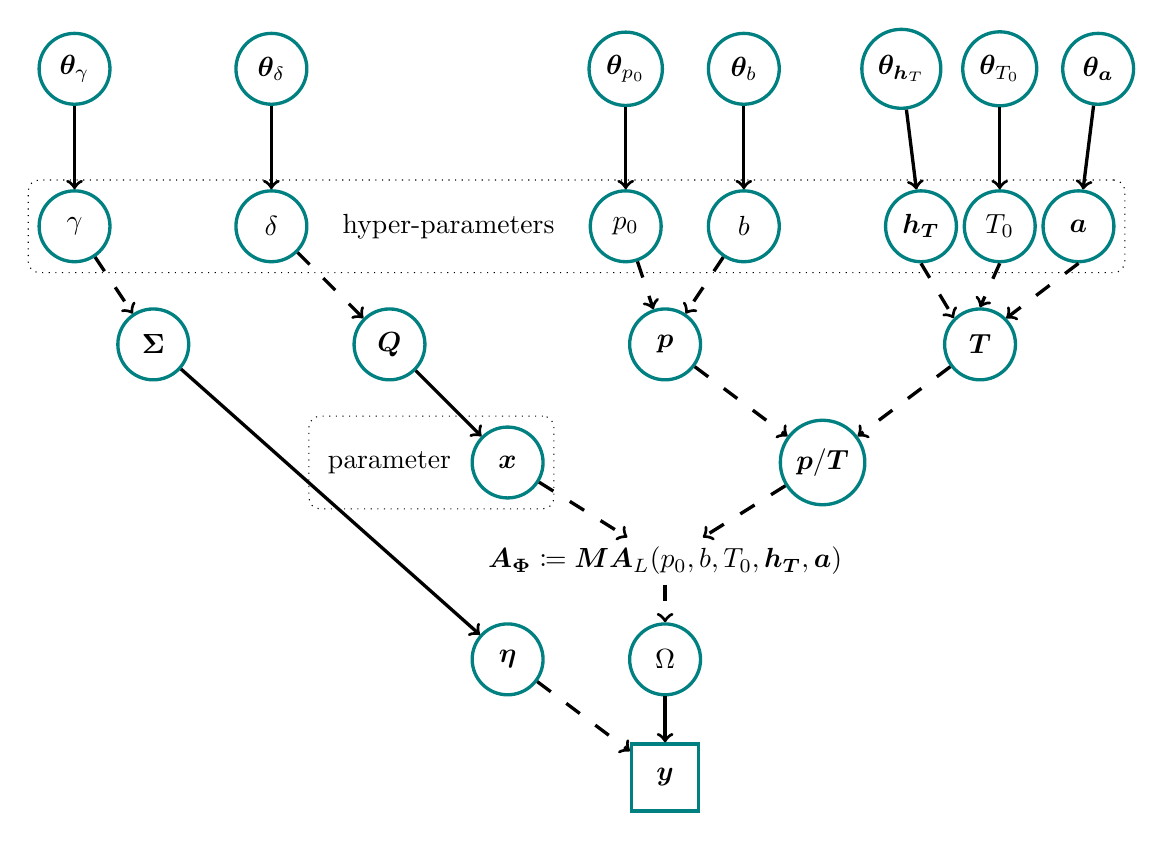
\begin{tikzpicture}
		\node[roundnode2] at (-4.5,6.5) (Q)     {$\bm{Q}$};
		\node[roundnode2] at (-3,5) (x)     {$\bm{x}$};
		\node[align=center] at (-1,3.75) (A)    {$\bm{A}_{\bm{\Phi}} \coloneqq \bm{M}\bm{A}_L(p_0,b,T_0,\bm{h_T},\bm{a})$};
		\node[roundnode2] at (-1,2.5) (u)    {$\Omega$};
		\node[rectnode] at (-1,1) (y)    {$\bm{y}$};
		\node[roundnode2] at (-3,2.5) (e)    {$\bm{\eta}$};
		\node[roundnode2] at (-7.5,6.5) (S)    {$\bm{\Sigma}$};
		\node[roundnode2] at (-8.5,8) (s)    {$\gamma$};
		\node[roundnode2] at (-6,8) (d)    {$\delta$};
		\node[roundnode2] at (3,6.5) (t)     {$\bm{T}$};
		\node[roundnode2] at (-1,6.5) (p)     {$\bm{p}$};
		\node[roundnode2] at (1,5) (pt)     {$\bm{p}/\bm{T}$};
		\node[roundnode2] at (0,8) (b1)    {$b$};
		%\node[roundnode2] at (1,8) (b2)    {$b_2$};
		%\node[roundnode2] at (-2,8) (h1)    {$h_{0}$};
		\node[roundnode2] at (-1.5,8) (p0)    {$p_0$};
		\node[roundnode2] at (2.25,8) (ht)    {$\bm{h_T}$};
		\node[roundnode2] at (3.25,8) (ct)    {$T_0$};
		\node[roundnode2] at (4.25,8) (at)    {$\bm{a}$};
		
		\node[roundnode2] at (0,10) (b1hyp)    {$\bm{\theta}_{b}$};
		%\node[roundnode2] at (-2.5,10) (h1hyp)    {$\bm{\theta}_{h_{0}}$};
		\node[roundnode2] at (-1.5,10) (p0hyp)    {$\bm{\theta}_{p_{0}}$};
		\node[roundnode2] at (2,10) (hthyp)    {$\bm{\theta}_{\bm{h}_T}$};
		\node[roundnode2] at (3.25,10) (cthyp)    {$\bm{\theta}_{T_{0}}$};
		\node[roundnode2] at (4.5,10) (athyp)    {$\bm{\theta}_{\bm{a}}$};
		
		\node[roundnode2] at (-8.5,10) (shyp)    {$\bm{\theta}_{\gamma}$};
		\node[roundnode2] at (-6,10) (dhyp)    {$\bm{\theta}_{\delta}$};
		
		%Lines
		
		
		\draw[->, very thick] (S) -- (e);
		\draw[->, mydotted, very thick] (s) -- (S);
		\draw[->, very thick] (u) -- (y);
		\draw[->, mydotted, very thick] (A) -- (u);
		\draw[->, mydotted,  very thick] (x) -- (A);
		\draw[->, mydotted, very thick] (p) -- (pt);
		\draw[->, mydotted, very thick] (t) -- (pt);
		\draw[->, mydotted, very thick] (pt) -- (A);
		%\draw[->, mydotted, very thick] (h1) -- (p);
		\draw[->, mydotted, very thick] (p0) -- (p);
		\draw[->, mydotted, very thick] (b1) -- (p); 
		%\draw[->, very thick] (b2.south) -- (p.east); 
		\draw[->, mydotted, very thick] (d) -- (Q); 
		\draw[->, mydotted, very thick] (e) -- (y); 
		
		\draw[->, very thick] (Q.south east) -- (x.north west); 
		\draw[->, mydotted, very thick] (ht.south) -- (t.north west);
		\draw[->, mydotted, very thick] (ct.south) -- (t.north);
		\draw[->, mydotted, very thick] (at.south) -- (t.north east);
		
		
		\draw[->, very thick] (b1hyp) -- (b1);
		%\draw[->, very thick] (h1hyp) -- (h1);
		\draw[->, very thick] (p0hyp) -- (p0);
		\draw[->, very thick] (hthyp) -- (ht);
		\draw[->, very thick] (cthyp) -- (ct);
		\draw[->, very thick] (athyp) -- (at);
		\draw[->, very thick] (shyp) -- (s);
		\draw[->, very thick] (dhyp) -- (d);
		
		\node[fit=(s)(at),draw,dotted,black, rounded corners] {};
		\node[align =center] at (-3.75,8) (T1) {hyper-parameters};
		\node[align =center] at (-4.5,5) (T2) {parameter};
		\node[fit=(x)(T2),draw,dotted,black, rounded corners] {};
		
	\end{tikzpicture} 
	\caption[Directed acyclic graph of Bayesian model for ozone $\bm{x}$, pressure $\bm{p}$ and temperature $\bm{T}$.]{DAG of the hierarchical Bayesian model including ozone $\bm{x}$, pressure $\bm{p}$ and temperature $\bm{T}$. The hyper-parameters $\bm{h}_T= \{ h_{T,1}, h_{T,2},h_{T,3},h_{T,4},h_{T,5},h_{T,6}\}$, $\bm{a} = \{ a_0, a_1, a_2,a_3,a_4,a_5,a_6\}$, $T_0$, $b$ and $p_0$ deterministically (dotted line) describe pressure through Eq.~\ref{eq:pressFunc} and temperature through Eq.~\ref{eq:tempFunc}. In this case, the hyper-parameters $\pi(p_0,b,T_0,\bm{h_T},\bm{a})$ are a normally distributed a-priori. That is why $\bm{\theta}_{\bm{h}_T},\bm{\theta}_{\bm{a}}, \bm{\theta}_{T_{0}},\bm{\theta}_{b} , \bm{\theta}_{p_0}$ represent means and STDs e.g.,~$b \sim \mathcal{N}(\mu_b, \sigma^2_b)$ and $\bm{\theta}_{b} = \{\mu_b, \sigma_b\}$.
		As previously described in Sec.~\ref{sec:BayModelO3}, $\bm{\theta}_{\gamma}, \bm{\theta}_{\delta}$ determine gamma distributions e.g., $\gamma \sim \mathcal{T}(\alpha_{\gamma},\beta_{\gamma}) $ with $\bm{\theta}_{\gamma} = 	\{\alpha_{\gamma},\beta_{\gamma} \}$.
		The ozone parameter $\bm{x}$ is statistically (solid line) described by the prior distribution $\bm{x}| \delta \sim \mathcal{N}(0,(\delta \bm{L})^{-1}) $. 
		Here, the hyper-parameter $\delta$ accounts for smoothness in the ozone profile and defines the precision matrix $\bm{Q} = \delta \bm{L}$ as in Eq.~\ref{eq:GLapl}.
		The approximated forward model $\bm{A}_{\bm{\Phi}} \coloneqq \bm{M}\bm{A}_L(p_0,b,T_0,\bm{h_T},\bm{a})$ with $\bm{\Phi}  \coloneqq \{p_0, b, T_0,\bm{h}_T,\bm{a} \}$ maps the parameter and hyper-parameters to a space of all measurables $\Omega$. 
		From that space, a data set $\bm{y}$ including some additive random noise $\bm{\eta}$ is observed (square box).
		The noise covariance $\bm{\Sigma} = \gamma^{-1} \bm{I}$ of the random noise vector $\bm{\eta} \sim \mathcal{N}(0,\gamma^{-1} \bm{I} ) $ is defined by the hyper-parameter $\gamma$.}
	%Given the data we like to determine the marginal posterior distribution over the hyper-parameters $\pi(\bm{\theta}, \delta, \gamma | \bm{y})$ first and then the conditional posterior distribution for ozone $\pi(\bm{x}|\bm{\theta}, \delta, \gamma, \bm{y})$, utilising the MTC scheme.}
\label{fig:DAGComplete}
\end{figure}
As in Sec.~\ref{sec:BayModelO3}, the DAG in Fig.~\ref{fig:DAGComplete} visualises the measurement process and conditional dependencies between the parameter and the hyper-parameters.
This hierarchical Bayesian framework includes the hyper-parameters $p_0, b$ for pressure (see Eq.~\ref{eq:pressFunc}), $\bm{a}, \bm{h}_T, T_0$ for temperature (see Eq.~\ref{eq:tempFunc}), $\delta$ for ozone smoothness and $\gamma$ for noise precision.
The hyper-parameters are described by the hyper-prior distribution $\pi(p_0,b,T_0,\bm{h_T},\bm{a}, \delta,\gamma)$ (see Sec.~\ref{subsec:PriorFull}).
Through their respective prior distributions, pressure $\bm{p}$, temperature $\bm{T}$ and ozone $\bm{x}$ progress deterministically (dashed line) into the forward model via $\bm{x} \times \bm{p} / \bm{T}$ and generate a space of all possible noise-free data $\Omega$.
Note that other variables in the RTE, such as the internal partition function and the black body radiation, are dependent on temperature (see Sec.~\ref{sec:RTE}).
From $\Omega$ we observe (square box) some data with additive normally distributed noise $\bm{\eta}$.
For brevity, we define the linear forward model matrix as
\begin{align}
\bm{A}_{\bm{\Phi}} \coloneqq \bm{M}\bm{A}_L(p_0,b,T_0,\bm{h_T},\bm{a}) 
\end{align}
with $\bm{\Phi}  \coloneqq \{p_0,b,T_0,\bm{h_T},\bm{a}  \}$ accounting for the all pressure and temperature related hyper-parameters and $\bm{M}$ is an affine approximation.
First $\bm{M} = \bm{I}$ is set to the identity matrix and after obtained results with a model given by the linearised RTE updated to an affine approximation mapping from the linearised RTE to the non-linear RTE.

The distributions of the hierarchical Bayesian framework are:
\begin{subequations}
\label{eq:BayMode}
\begin{align}
	\bm{y} |  \bm{x},\bm{\Phi},\delta,\gamma  &\sim \mathcal{N}(\bm{A}_{\bm{\Phi}}  \bm{x}, \gamma^{-1} \bm{I}) \label{eq:likelihoodFull} \\
	\bm{x}| \delta  &\sim \mathcal{N}(\bm{0}, (\delta \bm{L})^{-1} ) \label{eq:priorXFull} \\
	\delta  &\sim \mathcal{T}(\alpha_{\delta} , \beta_{\delta} )\label{eq:priorDelFull} \\
	\gamma  &\sim \mathcal{T}(\alpha_{\gamma}, \beta_{\gamma})\label{eq:priorGamFull} \\
	\bm{a}  &\sim \mathcal{N}(\bm{\mu}_{\bm{a}}, \bm{\Sigma}_{\bm{a}})\\
	\bm{h}_{\bm{T}}  &\sim \mathcal{N}(\bm{\mu}_{T}, \bm{\Sigma}_{\bm{h}_T}) \\
	T_0  &\sim \mathcal{N}(\mu_{T_0}, \sigma^2_{T_0} )\\
	p_0  &\sim \mathcal{N}(\mu_{p_0}, \sigma^2_{p_0} )\\
	b  &\sim \mathcal{N}(\mu_b, \sigma^2_b )  \label{eq:lastprior}  \, .
\end{align}
\end{subequations}
Due to Gaussian noise $\pi(\bm{y} |  \bm{x},\bm{\Phi},\delta,\gamma )$ is a normally distributed likelihood function and Eq.~\ref{eq:priorXFull} to Eq.~\ref{eq:lastprior} denote prior distributions.
Before formulating the posterior distribution, we carefully define $\bm{\theta}_{\gamma}, \bm{\theta}_{\delta},\bm{\theta}_{p_0},\bm{\theta}_{b},\bm{\theta}_{\bm{h}},\bm{\theta}_{T_0},\bm{\theta}_{\bm{a}}$, the hyper-prior scales, shapes, means and variances, which are explicitly given in Tab.~\ref{tab:priors}.


%Note that we fit one exponential function to ground truth pressure values between $h_{L,0} \approx 7$km and $h_{L,n} \approx 82$, so that the pressure value $p_0$ may be different to true sea-level pressure values at $h = 0$km due to that approximation.
\section{Posterior Distribution}
Here, the marginal posterior over the hyper-parameters $\bm{\theta} = \{ \bm{\Phi}, \gamma, \delta \}$ and the full conditional posterior distribution for the parameter $\bm{x}|\bm{\theta}$ are formulated.
To draw samples from the marginal posterior $\pi(\bm{\theta}| \bm{y})$ we utilise a TT approximation on a predefined grid to generate samples via the SIRT method with an MH correction step.
In doing so, the reader is guided through the process of obtaining an efficient higher-dimensional TT approximation.
Lastly, the RTO method is utilised to draw ozone samples from the full conditional posterior $\pi(\bm{x}|p_0,b,T_0,\bm{h_T},\bm{a} ,\delta, \gamma, \bm{y})$.
Recall that $\bm{x} \in \mathbb{R}^n$ with $n = 34$ and $\bm{y} \in \mathbb{R}^m$ with $m = 30$, and that the linear forward model matrix $\bm{A}_{\bm{\Phi}}$ is depending on the hyper-parameter defined as $\bm{\Phi}  \coloneqq \{p_0,b,T_0,\bm{h_T},\bm{a}  \}$.
Consequently, the marginal posterior is denoted as $\pi( \bm{\Phi},\delta,\gamma  | \bm{y}) $ and the full conditional posterior as $\pi(\bm{x}|\bm{\Phi}, \delta, \gamma, \bm{y})$.
\begin{table}[ht!]
\centering
\begin{tabular}{ |c||c|c|c|c|  }
	\hline
	& &\multicolumn{2}{|c|}{TT bounds}& \\
	\hline
	model parameters& priors&\makecell{lower}& \makecell{upper\\
	}&Context\\
	\hhline{|=||=|=|=|=|}
	$\bm{x}$ &$\mathcal{N}(0,(\delta \bm{L})^{-1})$ & -&-& $\bm{x}$\\ \hline
	$\delta$ &$\mathcal{T}(1,10^{-35})$ & -&-& $\bm{x}$\\ \hline
	$\gamma$ & $\mathcal{T}(1,10^{-35})$ &$8\times10^{14}$ &$1.2\times10^{16}$& $\bm{y}$\\ \hline
	$b$ &  $\mathcal{N}(0.174,(0.01)^2)$& 0.129& 0.214 &$\bm{p}$\\ \hline
	$h_{T,1}$ &  $\mathcal{N}(11,(1.5)^2)$&5.4 &16.3&$\bm{T}$\\ \hline
	$T_{0}$ &  $\mathcal{N}(288.15,(10)^2)$& 247 &326&$\bm{T}$\\ \hline
	$p_0$ &  $\mathcal{N}(1311,(20)^2)$&1237 &1387&$\bm{p}$\\ \hline
	$h_{T,3}$ &  $\mathcal{N}(32.3,(2.5)^2)$&22.9&41.7&$\bm{T}$\\ \hline
	$a_{1}$ &  $\mathcal{N}(0,(0.1)^2)$&-0.38 &0.38&$\bm{T}$\\ \hline
	$h_{T,2}$ &  $\mathcal{N}(20.1,(0.7)^2)$&17.2 &22.7&$\bm{T}$\\ \hline
	$a_{0}$ &  $\mathcal{N}(-6.5,(0.01)^2)$&-6.54 &-6.47&$\bm{T}$\\ \hline
	$a_{2}$ &  $\mathcal{N}(1,(0.01)^2)$&0.97 &1.03&$\bm{T}$\\ \hline
	$a_{3}$ &  $\mathcal{N}(2.8,(0.1)^2)$&2.5 &3.1&$\bm{T}$\\ \hline
	$h_{T,4}$ &  $\mathcal{N}(47.4,(0.5)^2)$&45.5 &49.3&$\bm{T}$\\ \hline
	$a_{4}$ &  $\mathcal{N}(0,(0.1)^2)$&-0.38 &0.38&$\bm{T}$\\ \hline
	$h_{T,5}$ &  $\mathcal{N}(51.4,(0.5)^2)$&49.5 &53.3&$\bm{T}$\\ \hline
	$a_{5}$ &  $\mathcal{N}(-2.8,(0.1)^2)$&-3.18 &-2.43&$\bm{T}$\\ \hline
	$h_{T,6}$ &  $\mathcal{N}(71.8,(3)^2)$&60.5 &83.1&$\bm{T}$\\ \hline
	$a_{6}$ & $\mathcal{N}(-2,(0.01)^2)$ &-2.04 &-1.96&$\bm{T}$\\
	\hline
\end{tabular}
\caption[Summary of relevant parameter characteristics, bounds and sampling statistics.]{Summary of relevant parameter and hyper-parameters bounds and statistics, ordered as in the TT format according to their correlation structure. We denote $\mathcal{N}(\mu= \text{mean},\sigma^2= \text{variance})$ as the Gaussian and $\mathcal{T}(\alpha = \text{scale}, \beta = \text{rate})$ as the Gamma distribution. The IACT $\tau_{\text{int}}$ from marginal posterior samples via the t-walk is twice the value provided by~\cite{UwerrM, drikHesse}.}
\label{tab:priors}
\end{table}
\clearpage

\subsection{Marginal Posterior -- Pressure and Temperature}
The marginal posterior is given as
\begin{align}
\pi( \bm{\Phi},\delta,\gamma  | \bm{y}) \propto &  \delta^{n/2} \gamma^{m/2}   \exp{ \Bigl\{ - \frac{1}{2} g ( \bm{\Phi},\delta,\gamma ) - \frac{\gamma}{2} f (\bm{\Phi},\delta,\gamma ) \Bigr\}} \pi(\bm{\Phi},\delta,\gamma ) \, ,
\label{eq:MargPostFull}
\end{align}
with,
\begin{subequations}
\label{eq:fandgTrue}
\begin{align}
	&f ( \bm{\Phi},\delta, \gamma) = \bm{y}^T \bm{y} - \big(\bm{A}_{\bm{\Phi}}^T \bm{y}\big)^T \big(\gamma \bm{A}_{\bm{\Phi}}^T  \bm{A}_{\bm{\Phi}} + \delta \bm{L}\big)^{-1} \big(\bm{A}_{\bm{\theta}}^T \bm{y}\big)  \label{eq:fFullAppl} \, ,  \\
	&\text{and } g(\bm{\Phi},\delta, \gamma) = \log \det \big(\gamma \bm{A}_{\bm{\Phi}}^T  \bm{A}_{\bm{\Phi}} + \delta \bm{L}\big) \label{eq:gFullAppl} \, .
\end{align}
\end{subequations}
For each evaluation of $\pi( \bm{\Phi},\delta,\gamma  | \bm{y})$, $\bm{A}_{\bm{\Phi}}$ is composed as in Chapter~\ref{ch:formodel}, and $f$ and $g$ are calculated directly using the Cholesky decomposition via the Python functions \texttt{numpy.linalg.cholesky} and \texttt{scipy.linalg.cho\_solve}.

\subsection{Posterior Distribution}
\label{sec:FirstO3Post}
As explained in Sec.~\ref{subsec:TheoMTC}, we factorise the posterior
\begin{align}
	\pi( \bm{x},\bm{\Phi}, \delta, \gamma| \bm{y}) \propto \pi(\bm{y}| \bm{x},\bm{\Phi},\delta,\gamma) \pi( \bm{x},  \bm{\Phi},\delta,\gamma)
\end{align}
into 
\begin{align}
	\pi( \bm{x}, \bm{\Phi}, \delta,\gamma| \bm{y}) =\pi( \bm{x}| \bm{\Phi},\delta,\gamma, \bm{y})\pi( \bm{\Phi},\delta,\gamma | \bm{y})
\end{align}
the marginal posterior $\pi(\bm{\Phi},\delta ,\gamma| \bm{y})$ and full conditional posterior $\pi( \bm{x}| \bm{\Phi},\delta,\gamma, \bm{y})$ (see Eq.~\ref{eq:MTC}).
%Fox and Norton call this method the marginal and then conditional method (MTC) \cite{fox2016fast}, where we break the correlation structure between $\bm{x}$ and $\gamma, \delta$ as illustrated in Fig. \ref{fig:RueHeld} by marginalising over $\bm{x}$.
As discussed in~\cite{fox2016fast}, for the linear-Gaussian case, $\bm{x}$ cancels in the marginal posterior over the hyper-parameters.
Following the MTC scheme, we characterise the marginal posterior first and then the full conditional posterior.

\subsubsection{Full Conditional Posterior}
\label{subsec:firstCond}
As in \cite{SIMPSON201216}, consider the joint Gaussian distribution
\begin{align}
	\begin{pmatrix}
		\bm{x} \\
		\bm{y}
	\end{pmatrix}\sim \mathcal{N}\left[  \begin{pmatrix}
		\bm{\mu} \\
		\bm{A}\bm{\mu}
	\end{pmatrix},\begin{pmatrix}
		\bm{Q}_{\bm{\theta}} + \bm{A}_{\bm{\Phi}}^T \bm{\Sigma}_{\bm{\theta}}^{-1} \bm{A}_{\bm{\Phi}} & - \bm{A}_{\bm{\Phi}}^T \bm{\Sigma}_{\bm{\theta}}^{-1} \\
		\bm{\Sigma}_{\bm{\theta}}^{-1} \bm{A}_{\bm{\Phi}} & \bm{\Sigma}_{\bm{\theta}}^{-1} 
	\end{pmatrix}^{-1} \right] \, 	\label{eq:jointMultiGaus}
\end{align}
with $\bm{\Sigma}_{\bm{\theta}}^{-1} = \gamma \bm{I} $ and $\bm{Q}_{\bm{\theta}}  = \delta \bm{L} $ and $\bm{\mu} = \bm{0}$.
Then the full conditional posterior distribution of ozone 
\begin{align}
	\bm{x}|\bm{\Phi}, \delta, \gamma, \bm{y}  \sim \mathcal{N}\big(  (\bm{A}_{\bm{\Phi}}^T \bm{A} + \delta / \gamma \bm{L} )^{-1} \bm{A}_{\bm{\Phi}}^T \bm{y}, (  \gamma \bm{A}_{\bm{\Phi}}^T \bm{A}_{\bm{\Phi}} + \delta \bm{L}  \big) \, \label{eq:CondPost},
\end{align}
is a normal distribution and samples can be drawn via the randomise then optimise (RTO) method (see Sec.~\ref{subsec:FullCondPost}).


\section{Results}
In this section the results are presented.
Given the data see Sec. the inverse problem is treated as a linear inverse problem by neglecting the non-linear absorption in the RTE.
Then an affine approximation is found and the non-linear forward model is approximated by the affine map and the linear forward model.
Finally, we present posterior ozone, pressure and temperature profiles based on the approximated forward model.

\subsection{Linear Forward Model}

Here as already mentioned the forward model is defined as:
\begin{align}
	\bm{A}_{\bm{\Phi}} \coloneqq \bm{A}_L(p_0,b,T_0,\bm{h_T},\bm{a}) \, .
\end{align}

Consequently, with the priors and simulated data, the marginal and conditional posterior are well defined and a Tensor-Train approximation of the marginal posterior is approximated using a tensor-train (TT) and the squared inverse Rosneblatt transport (SIRT) \cite{} is employed to generate samples from the marginal posterior.
Conditioned on those samples the randomise then optimise (RTO) method \cite{} is used to sample from the full conditional posterior.

\subsubsection{Tensor-Train Approximation of the Marginal Posterior}
Instead of using conventional Markov-Chain Monte-Carlo methods to generate samples from the marginal posterior, we approximate the marginal posterior directly using a TT representation.
In the following a brief introduction to the TT format is provided.

Assume the target function is $\pi( \bm{\Phi},\delta,\gamma  | \bm{y})$ and the parameter $\bm{\theta} \coloneqq \{\bm{\Phi},\delta,\gamma  \} \in \mathbb{R}^d  $ is $d$-dimensional.
First a $d$-dimensional grid with $n$ grid points in for dimension in the parameter space has to be defined.
So a TT represents a parameter space $n^d$ grid points.
Since that is computationally not feasible a TT is employed to approximate that space.
More specifically, to ensure non-negativity, we approximate the square root of $\pi( \bm{\theta}  | \bm{y})$ over the whole parameter space can be written as:
\begin{align}
	\sqrt{\pi( \bm{\theta}  | \bm{y})} \approx \tilde{g}(\bm{\theta}) =  \bm{G}_1(\theta_1), \dots, \bm{G}_k(\theta_k), \dots, \bm{G}_d(\theta_d)\, .
\end{align}
where each $\bm{G}_k \in \mathbb{R}^{r_{k-1}\times n \times r_{k}}$ is a TT core.
Further, $r_{k}$ are the ranks of the individual cores and bounded by $r_{0} = 1$ and $r_{d} = 1$.
For now assume the ranks $r_k = r$ for $k =1, \dots, d-1$, then the TT approximates the function space with $n \times r^2 \times (d-2) + n \times r \times 2$ function evaluations instead of the $n^d$ function evaluations traditionally required.
To generate a TT for $\sqrt{\pi( \bm{\theta}  | \bm{y})}$ we use the \textcolor{red}{toolbox}, which implements the TT-Cross algorithm from \cite{}.

Given a TT approximation samples from the target function are generated via the inverse Rosenblatt transport (IRT) scheme \cite{}.
Because each of the TT cores is representative for one dimensions in the parameter it is easy to integrate over the individual parameter dimensions.
This way a sequence of 1-dimensional functions can be constructed, so that
\begin{align*}
		\pi( \bm{\theta}  | \bm{y}) =&  \quad \pi(\theta_1 | \bm{y}) \\
			& \quad \times \pi( \theta_2 | \theta_1, \bm{y}) \\
			&\quad \times\pi( \theta_3 | \theta_2,\theta_1, \bm{y})  \\
			&\quad \times\pi( \theta_4 | \theta_3, \theta_2,\theta_1, \bm{y}) \\
			& \quad \quad \vdots \\
			&\quad \times \pi( \theta_d | \theta_{d-1}, \dots, \theta_4,\theta_3, \theta_2,\theta_1, \bm{y}) \, .
\end{align*}
For each one-dimensional 'conditional marginal' $\pi( \theta_k | \theta_{k-1},\dots, \theta_1, \bm{y})$ conditioned on $\theta_{k-1},\dots, \theta_1, $ and marginalised over $\theta_{k+1} , \dots, \theta_d$  a mapping from the uniform distribution is constructed via the cumulative distribution function (CDF)
\begin{align}
	F(\theta_k) = \int_{-\infty}^{\theta_k} \pi( \hat{\theta}_k | \theta_{k-1},\dots, \theta_1, \bm{y}) \diff \hat{\theta}_k  \, .
	\label{eq:CurrCDF}
\end{align}
Then a uniformly distribute random variable $\bm{u} \sim \mathcal{U} [0,1]$ is projected onto the parameter space via the inverse
\begin{align*}
	\theta_k = F^{-1}(u_k)
\end{align*}
with $u_k \in \bm{u}$.

Since we approximate the square root of the target function this is the squared inverse Rosneblatt transport (SIRT), where a small constant $\xi$ is added so that \begin{align}
	\pi( \bm{\theta}  | \bm{y}) \approx \xi +  \tilde{g}(\bm{\theta})
\end{align}
This ensure positivity and makes each of the well defined.
See \cite{} on how to calculate each of the conditional marginals in practise.




What is a tensor-train?
What do we approximate?
How do sample?
What grid to we choose?
How do we choose the ranks?


\subsubsection{Randomise then Optimise Method to Draw Samples from the Full Conditional Posterior}

In theory, this scheme provides independent samples, but in practice, every system produces correlated samples.
To assess how efficient this scheme is, we define the Integrated Autocorrelation Times (IACT)
\begin{align}
	\tau_{\text{int}}  \coloneqq  \Bigg(  1 + 2 \sum_{t = 1}^{W} \frac{\Gamma(t)}{\Gamma(0)}  \Bigg)  
\end{align} 
as in \cite{fox2016fast} with an autocorrelation coefficient $\Gamma(t)$.
This is twice the value of the IACT in~\cite[pp. 103-105]{wolff2002LecNot} and~\cite{wolff2004monte,drikHesse}, as commonly defined within the physics community.
U. Wolff~\cite{wolff2004monte} (and the Python implementation by D. Hesse~\cite{drikHesse}) provide a way to not only calculate the IACT safely but also to quantify the errors of the estimated IACT.
The IATCs are $\tau_{\text{int},\lambda} = 1.05\pm0.04$ and $\tau_{\text{int},\gamma} =0.99\pm0.03$ based on a chain with 10000 samples.
So every second sample via the IRT scheme presents an independent marginal posterior sample.
Conditioned on an independent sample from the marginal posterior, one can draw an independent sample from the full conditional posterior.

\subsection{Finding an Affine Map}
\label{sec:affine}
We find an affine map by creating the vector spaces $\bm{W}$ based on the linear forward model and $\bm{V}$ based on the non-linear forward model with ground truth pressure and temperature.
More specifically $m-1$ samples $\bm{x}^{(j)} \sim \pi_{\bm{x}}(\cdot|\delta^{(j)} , \gamma^{(j)},\bm{y})$, for $j = 2, \dots,m$, from the posterior and the posterior mean $\bm{\mu}_{\bm{x}|\bm{y}}$ generate,
\begin{align*}
	\bm{W} = \begin{bmatrix}
		\vert& \vert&   &  \vert & & \vert \\
		\bm{A}_{L}  \bm{\mu}_{\bm{x}|\bm{y}} & \bm{A}_{L}  \bm{x}^{(2)}   &  \cdots& \bm{A}_{L} \bm{x}^{(j)} &  \cdots & \bm{A}_{L} \bm{x}^{(m)} \\
		\vert& \vert&   &  \vert & & \vert 
	\end{bmatrix}
	\in \mathbb{R}^{m \times m}
\end{align*}\noindent and
\begin{align*}
	\bm{V} = \begin{bmatrix}
		\vert& \vert&   &  \vert & & \vert \\
		\bm{A}(\bm{\mu}_{\bm{x}|\bm{y}} ) & \bm{A}(\bm{x}^{(2)}) &  \cdots& \bm{A}(\bm{x}^{(j)}) &  \cdots & \bm{A} (\bm{x}^{(m)})  \\
		\vert&\vert&   &  \vert & & \vert 
	\end{bmatrix} = 
	\begin{bmatrix}
		\begin{array}{ccc}
			\horzbar & v_{1} & \horzbar \\
			& \vdots    &          \\
			\horzbar & v_{j} & \horzbar \\
			& \vdots    &          \\
			\horzbar &v_{m} & \horzbar
		\end{array}
	\end{bmatrix}\in \mathbb{R}^{m \times m} \, .
\end{align*}
Then the non-linear forward model is approximated as 
\begin{align}
	\bm{A}(\bm{x}) \approx \bm{M A}_L \bm{x} \, , \label{eq:AffineM}
\end{align}
where we solve $v_j =r_j \bm{W}$ for each row $r_j$ in
\begin{align*}
	\bm{V}\bm{W}^{-1} = \bm{M} =
	\begin{bmatrix}
		\begin{array}{ccc}
			\horzbar & r_{1} & \horzbar \\
			& \vdots    &          \\
			\horzbar & r_{j} & \horzbar \\
			& \vdots    &          \\
			\horzbar &r_{m} & \horzbar
		\end{array}
	\end{bmatrix}\, \in \mathbb{R}^{m \times m} .
\end{align*}
using the Python function \texttt{numpy.linalg.solve}.
This is feasible since every noise-free measurement is independent of each other, and then every row $v_j$ of $\bm{V} \in \mathbb{R}^{m \times m}$ is independent of each other as well.
For an $\bm{x} = \bm{\mu}_{\bm{x}|\bm{y}} + \Delta \bm{x}$ we rewrite Eq.~\ref{eq:AffineM} to
\begin{align}
	\bm{A}(\bm{x})  \approx \underbrace{  \bm{M A}_L  \bm{\mu}_{\bm{x}|\bm{y}} }_{= \bm{A}( \bm{\mu}_{\bm{x}|\bm{y}} )  }+  \underbrace{\bm{M A}_L  \Delta \bm{x} }_{= \bm{A}^{\prime}( \bm{\mu}_{\bm{x}|\bm{y}} )  \Delta \bm{x} }\, \\
	=    \underbrace{ \bm{A}^{\prime}( \bm{\mu}_{\bm{x}|\bm{y}} ) \bm{x}}_{ \bm{A}\bm{x}}  +  \underbrace{ \bm{A}( \bm{\mu}_{\bm{x}|\bm{y}} )  - \bm{A}^{\prime}( \bm{\mu}_{\bm{x}|\bm{y}} ) \bm{\mu}_{\bm{x}|\bm{y}}}_{  \bm{b}}
\end{align}
to show that $ \bm{M}:\bm{A}_L\bm{x} \rightarrow \bm{A}(\bm{x})$ is an affine map.

\begin{figure}[ht!]
	\centering
	%\includegraphics{AffinePapAssMap.png}
	\caption[Assessment of affine map.]{Assessment of how well the affine map $\bm{M}$ approximates noise-free non-linear data $\bm{A}(\bm{x})$ (red circles) from noise-free linear data $\bm{A}_L\bm{x}$ (grey stars). The approximated noise-free data (black stars) has a relative RMS error of $\approx 0.01\%$ compared to the true non-linear noise-free data.
		The ozone profile $\bm{x}$ to generate this noise-free data has not been used to create the affine map.}
	\label{fig:AssMap}
\end{figure}
The relative RMS difference $\lVert \text{vec}(\bm{M}\bm{W}) - \text{vec}(\bm{V})  \rVert_{L^2} / \lVert \text{vec}(\bm{M}\bm{W}) \rVert_{L^2} $ between the mapped linear noise-free data and the non-linear noise-free data is approximately $0.001\%$.
This is much smaller than the relative RMS difference between $\bm{W}$ and $\bm{V}$ of about $1\%$.
Here $\text{vec}(\bm{V})$ vectorises the matrix $\bm{V}$.
Fig.~\ref{fig:AssMap} shows the mapping for one posterior ozone sample with a relative RMS error~$\approx0.01\%$.
This posterior ozone sample has not been used to create this mapping; in other words, this is an unseen event not occurring in the training data.
Consequently, from here onwards the approximated forward map is used.
This takes $\approx 0.1$s.


\subsection{Approximated Forward Model}

\begin{itemize}
	\item marginal posterior same TT setup
	\item conditional posterior
	\item plot results
\end{itemize}
\clearpage
\section{Conclusion}
\begin{itemize}
    \item TT approximation vs conventional sampler cite Rosenthal for IACT
    \item Pressure Ozone correlation
    \item 2nd Ozone peak not included 
\end{itemize}
\clearpage
% {\renewcommand*\MakeUppercase[1]{#1}%
% 	\printbibliography[heading=bibintoc,title={\bibtitle}]}
\printbibliography[heading=bibintoc,title={\bibtitle}]

\end{document}
